%%%%%%%%%%%%%%%%%%%% Documentación del sistema %%%%%%%%%%%%%%%%%%%%


\section{Documentación de sistema}

\subsection{Especificación del sistema}

\subsubsection{División de los módulos}

Aquí, se puede ver en cuántos subproblemas, hemos dividido el programa, y los módulos que van asociados a cada uno de ellos.
Las especificaciones de cada una de las funciones se puede encontrar en \href{DOC_DOXYGEN/index.html}{Doxygen} o en el apartado \ref{fig:CodigoModulos}.


\begin{center}
  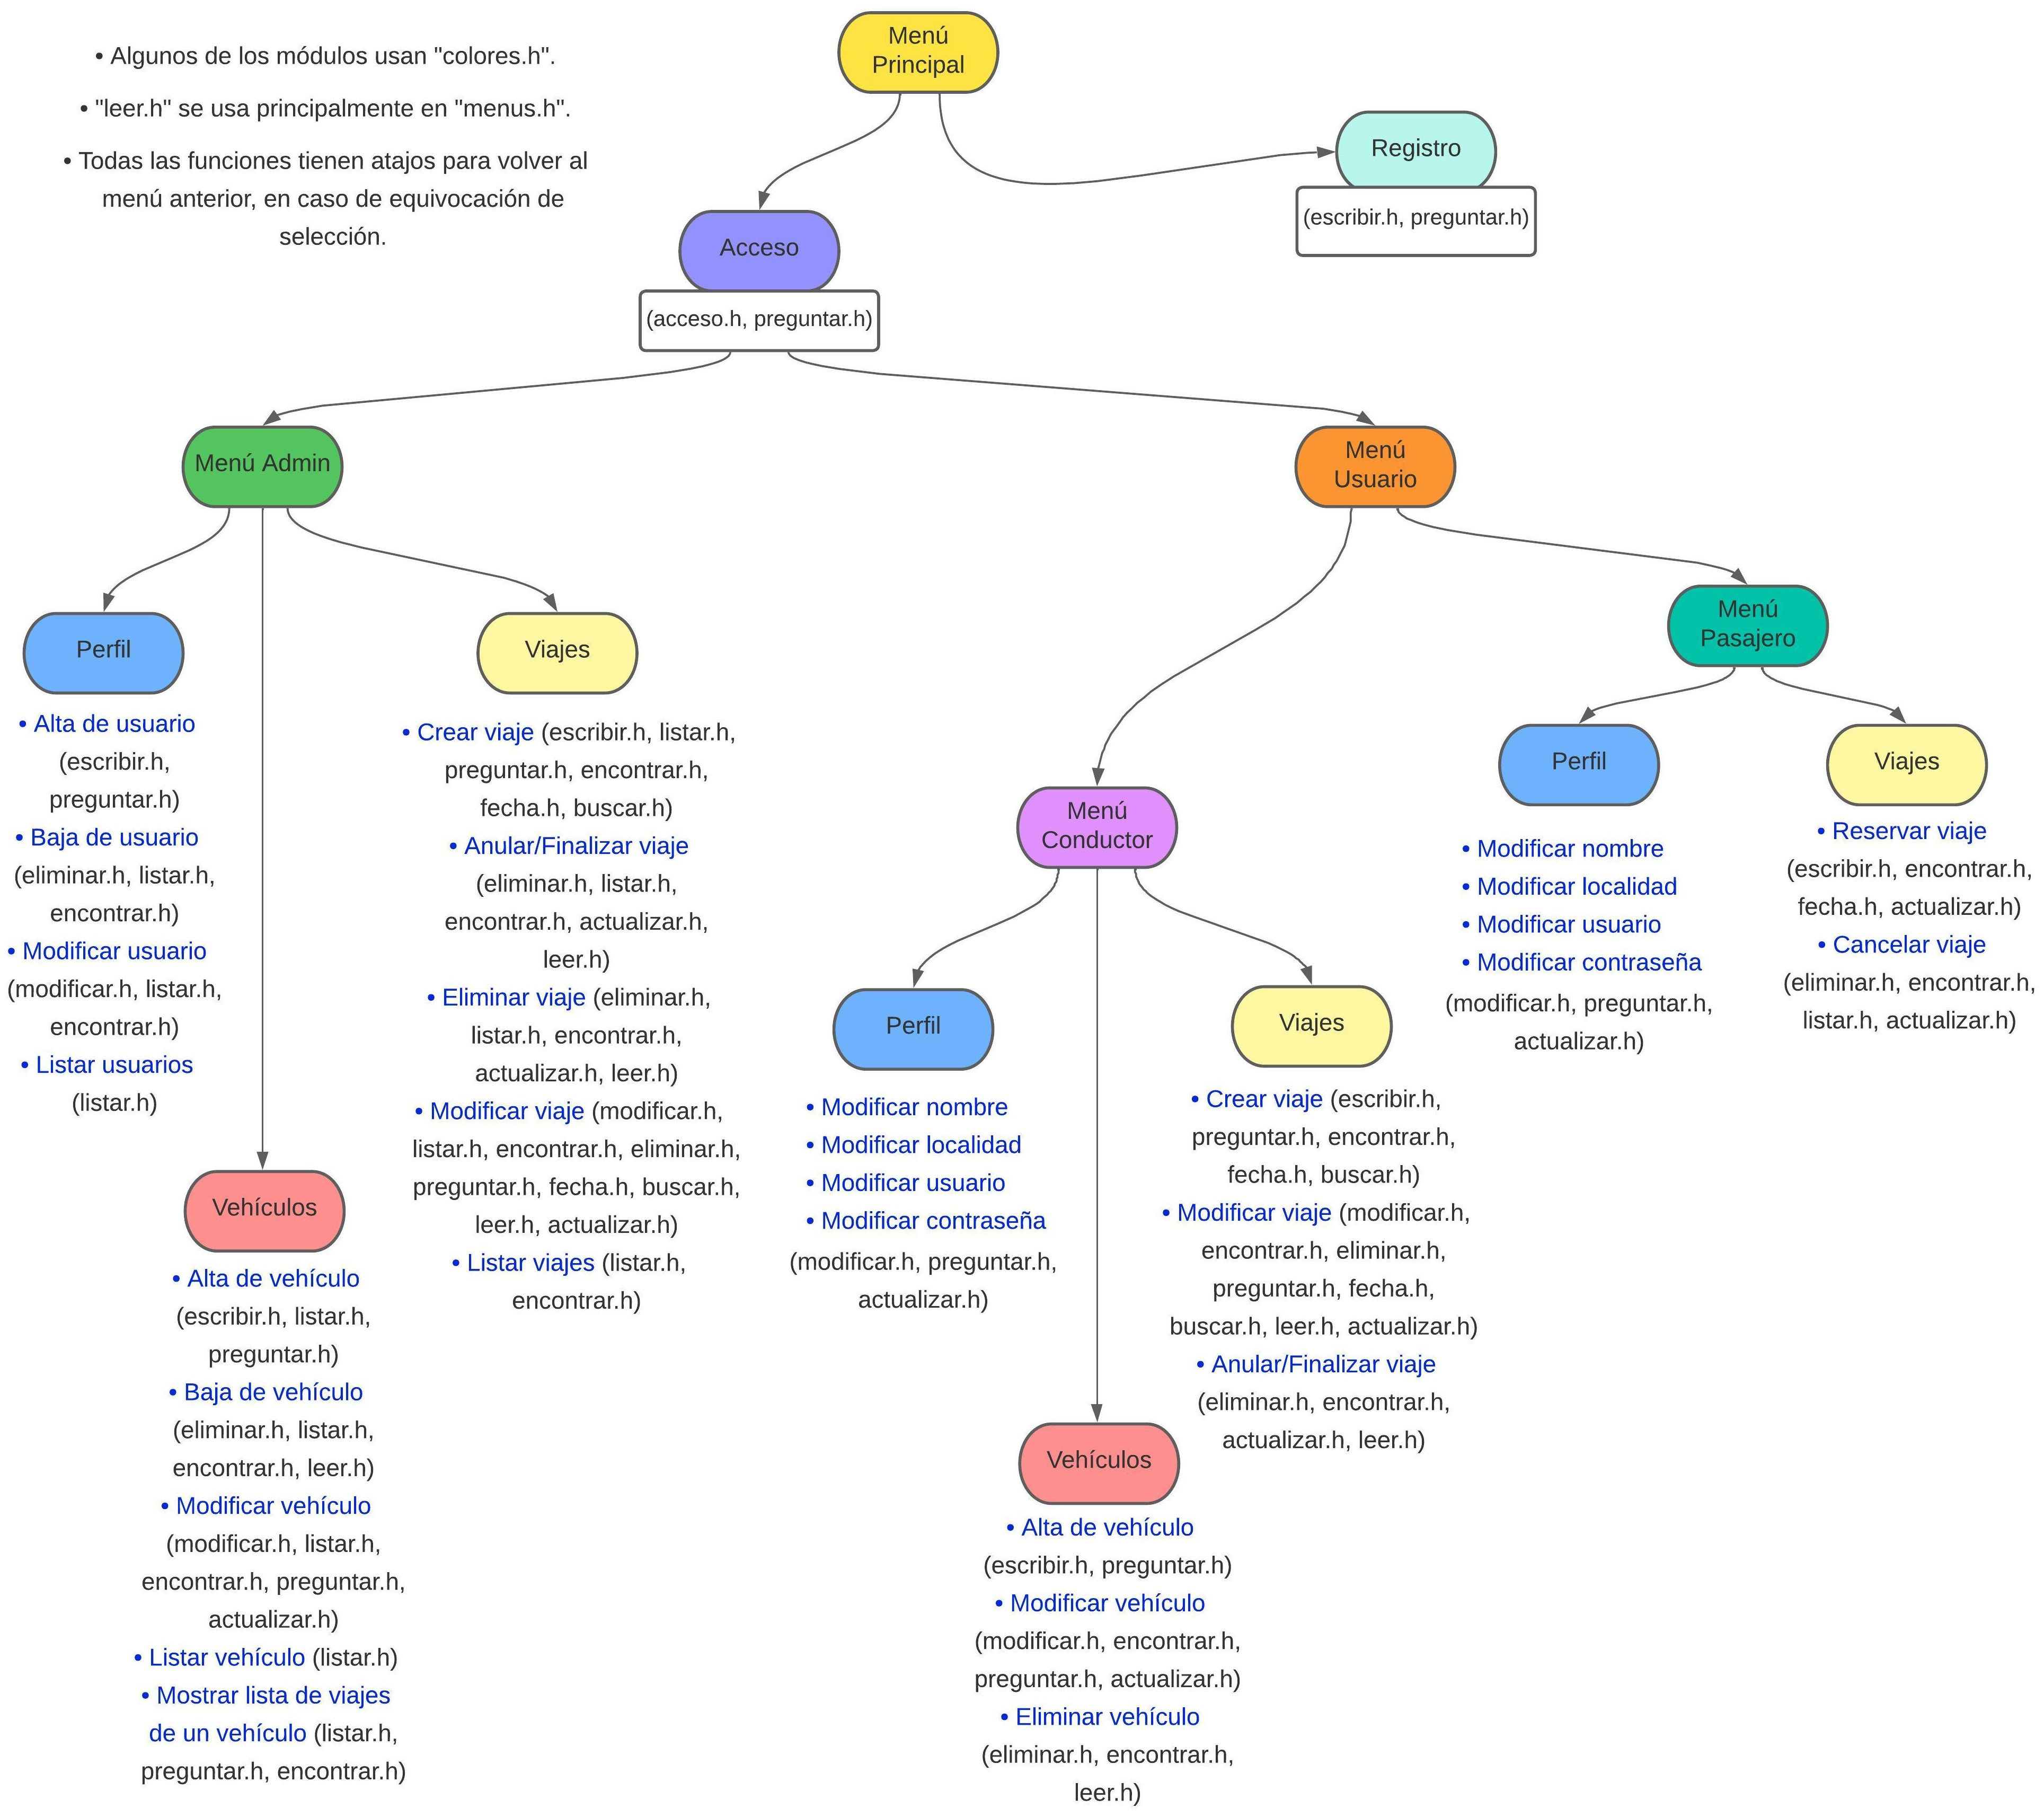
\includegraphics[width=1.15\textwidth]{FOTOS/Organigrama_Proyecto.jpeg}
\end{center}

Puede ver la imagen completa en \href{FOTOS/Organigrama_Proyecto.jpeg}{Organigrama Proyecto}.

\subsubsection{Relaciones de los módulos}

Aquí, puede ver la organización de la descomposición modular del proyecto, es decir, la forma en la que están emparejados los módulos,
para hacer que el programa funcione correctamente, y de la forma más óptima posible.\\
\begin{center}
  \includegraphics[width=1.1\textwidth]{FOTOS/Descomposicion_Modular.jpeg}
\end{center}

Puede ver la imagen completa en \href{FOTOS/Descomposicion_Modular.jpeg}{Descomposición Modular}.\\

\subsubsection{Plan de desarrollo del Software}

\bigskip

\begin{tabular}{|p{2.5cm}|p{8cm}|p{2cm}|}
  \hline
  \textbf{Fase} & \textbf{Descripción} & \textbf{Duración} \\
  \hline
  Análisis & Se dividen todos los problemas en subproblemas, para planificar todos los requisitos que necesita cada función para que cumpla los objetivos. & 1 semana \\
  \hline
  Desarrollo & Creamos todas las funciones, para que el programa haga lo que queramos. & 3 semanas \\
  \hline
  Optimización & Tratamos de ver si hay partes del código que se puedan sustituir por funciones ya existentes, para reusar código, y hacer que el programa sea más liviano. & 1 semana \\
  \hline
  Pruebas & Testeamos cada función y módulo por separado, para más tarde probarlo como un todo, y checkear si el proyecto es funcional, si no es así, hay que arreglar los errores. & 2 semanas \\
  \hline
  Documentación & Una vez que se ha realizado todo, se van incluyendo las especificaciones de las funciones, al igual que se agregan comentarios al código. & 1 semana \\
  \hline
\end{tabular}

\bigskip

Tras haber pasado todas estas fases, el programa está totalmente preparado para ser distribuido a los usuarios, en este caso, los miembros de la comunidad universitaria de la ESI,
es por esto que se pasa a una fase de Mantenimiento y Actualización, en la que se arreglan los errores que pueda tener el programa en las máquinas externas,
al igual que se van incluyendo actualizaciones para hacer que el programa tenga más funcionalidades, como por ejemplo, una creación de un sistema de valoraciones, a la hora de acabar un viaje.

\subsection{Módulos}

En este proyecto, se ha empleado una descomposición por tareas, por lo que el programa se ha dividido en 14 módulos, que son:

\subsubsection{Acceso}

Usado para darle acceso a los usuarios al sistema, mediante la autenticación de las credenciales que introduzcan.
Para esto se han usado algunos mecanismos interesantes, como la detección automática del perfil del usuario, si el que inicia sesión es usuario ó administrador.
Además, se ha implementado un sistema de seguridad, con el que el usuario solamente se dispone 3 intentos para introducir la contraseña.\\

Para ver el código fuente del módulo puede ir a \ref{fig:AccesoCod}, o entrar en \href{DOC_DOXYGEN/acceso_8h_source.html}{Doxygen}.
\label{fig:Acceso}

\subsubsection{Actualizar}

Sirve para reescribir todos los datos de la estructura en el fichero, y así sincronizarlos, por si se ha producido alguna modificación.\\

Para ver el código fuente del módulo puede ir a \ref{fig:ActualizarCod}, o entrar en \href{DOC_DOXYGEN/actualizar_8h_source.html}{Doxygen}.
\label{fig:Actualizar}

\subsubsection{Buscar}

Empleado para buscar todas las rutas posibles, que hay desde la ciudad que el usuario haya seleccionado
hasta la ESI, para hacer que no se repitan todas las rutas, se usa otra matriz, donde se introduce la ruta impresa, para comprobar que no se haya escrito en pantalla anteriormente,
y sólo listar las rutas no repetidas, y así ahorrar tiempo al usuario a la hora de crear un viaje. Una vez que el usuario selecciona la ruta, se escriben
todos los pasos en el fichero correspondiente.\\

Para ver el código fuente del módulo puede ir a \ref{fig:BuscarCod}, o entrar en \href{DOC_DOXYGEN/buscar_8h_source.html}{Doxygen}.
\label{fig:Buscar}

\subsubsection{Colores}

Gracias a este módulo se puede cambiar el fondo y el cuerpo del texto, dándole así algo de formato al proyecto.\\

Para ver el código fuente del módulo puede ir a \ref{fig:ColoresCod}, o entrar en \href{DOC_DOXYGEN/colores_8h_source.html}{Doxygen}.
\label{fig:Colores}

\subsubsection{Eliminar}

Utilizado para suprimir cualquier vehículo, viaje, paso o reserva. Cuando se le pregunta al usuario, qué vehículo quiere quitar de todos los que tiene,
y él selecciona uno, se eliminan todos sus viajes, pasos y reservas. Algo similar ocurre con los viajes, que se eliminan sus pasos y reservas.\\

Para ver el código fuente del módulo puede ir a \ref{fig:EliminarCod}, o entrar en \href{DOC_DOXYGEN/eliminar_8h_source.html}{Doxygen}.
\label{fig:Eliminar}

\subsubsection{Encontrar}

Se ha usado para buscar todos los vehículos, viajes o reservas que tiene un usuario. Con esto podemos saber cuántos viajes
tiene con un cierto estado o si se han ocupado plazas en el viaje, para así darle la posibilidad al usuario de anular, finalizar o modificar un viaje.
Todo esto, se devuelve en un vector de enteros dinámico, que indica la posición del vehículo, viaje o reserva en su respectiva estructura.\\

Para ver el código fuente del módulo puede ir a \ref{fig:EncontrarCod}, o entrar en \href{DOC_DOXYGEN/encontrar_8h_source.html}{Doxygen}.
\label{fig:Encontrar}

\subsubsection{Escribir}

Sirve para registrar usuarios, vehículos, viajes o reservas. Se han hecho algunas comprobaciones para que cuando se cree un usuario, no se pueda repetir de usuario,
o a la hora de registrar un vehículo, que se vea si la matrícula está bien introducida, con sus 4 números y 3 letras, y que no esté registrada en el sistema.
Además, en la parte de reservar un viaje, sólo se podrá hacer si pasa algún viaje por la localidad de residencia, en la fecha establecida por el usuario,
si hay viajes pero en otra fecha, se le avisará al usuario, si reserva, se eliminará una plaza del viaje.\\
Se ha creado una característica interesante, que es la reutilización de IDs, cuando se quiere crear un usuario, o un viaje, con esto si se elimina un usuario,
se podrá volver a crear otro con esa misma ID, ya que al suprimir un usuario, se quita todo el contenido que haya sobre el mismo en todos los ficheros.\\

Para ver el código fuente del módulo puede ir a \ref{fig:EscribirCod}, o entrar en \href{DOC_DOXYGEN/escribir_8h_source.html}{Doxygen}.
\label{fig:Escribir}

\subsubsection{Estructuras}

En este módulo, se han definido las estructuras necesarias para poner en marcha el proyecto.\\

Para ver el código fuente del módulo puede ir a \ref{fig:EstructurasCod}, o entrar en \href{DOC_DOXYGEN/annotated.html}{Doxygen}.

\label{fig:Estructuras}

\subsubsection{Fecha}

Gracias a este módulo se puede pedir una fecha, comprobando si la fecha y la hora es posterior a la actual, y si al introducir una hora de partida,
esta hora es posterior a la de llegada. Asimismo, se ha creado una función que compruebe todos los viajes que hay, y si alguno ha pasado la hora de inicio, se pone en estado "Iniciado",
mientras que si se ha excedido una hora desde la hora de llegada, se establecerá en estado "Finalizado", y se eliminarán sus pasos y reservas.\\

Para ver el código fuente del módulo puede ir a \ref{fig:FechaCod}, o entrar en \href{DOC_DOXYGEN/fecha_8h_source.html}{Doxygen}.
\label{fig:Fecha}

\subsubsection{Leer}

Usado para leer todos los ficheros que hay en la carpeta DATA e introducir la información escaneada en las estructuras creadas. Todo esto se puede hacer gracias a la función strtok,
que va rompiendo cada línea del fichero, hasta donde esté el carácter que queramos, en nuestro caso "-".
También, se ha creado un contador, para usarlo como delimitador en los bucles de otras funciones.\\

Para ver el código fuente del módulo puede ir a \ref{fig:LeerCod}, o entrar en \href{DOC_DOXYGEN/leer_8h_source.html}{Doxygen}.
\label{fig:Leer}

\subsubsection{Listar}

Creado con el objetivo de imprimir por pantalla listas de todos los usuarios, vehículos ó viajes que hay en el sistema.
También se ha creado para listar todas las localidades que hay en la provincia de Cádiz, al igual que puede escribir todos los vehículos, viajes o reservas que tiene un usuario.\\

Para ver el código fuente del módulo puede ir a \ref{fig:ListarCod}, o entrar en \href{DOC_DOXYGEN/listar_8h_source.html}{Doxygen}.
\label{fig:Listar}

\subsubsection{Menús}

En este módulo están todas las funciones que muestran por pantalla los menús, haciendo de puente entre las diferentes funciones de los demás módulos.
Se han creado varias interfaces, una para los Pasajeros, otra para los Conductor, y una tercera para el Administrador.\\

Para ver el código fuente del módulo puede ir a \ref{fig:MenusCod}, o entrar en \href{DOC_DOXYGEN/menus_8h_source.html}{Doxygen}.
\label{fig:Menus}

\subsubsection{Modificar}

Sirve para cambiar cualquier dato de un vehículo o viaje de un usuario, e incluso para rectificar los datos personales del usuario, o actualizar la contraseña.\\

Para ver el código fuente del módulo puede ir a \ref{fig:ModificarCod}, o entrar en \href{DOC_DOXYGEN/modificar_8h_source.html}{Doxygen}.
\label{fig:Modificar}

\subsubsection{Preguntar}

Utilizado para escanear cadenas, cambiando el carácter de salto de línea por el carácter nulo. Además se ha usado para preguntar una contraseña,
empleando * para ocultarla, y haciendo que si la contraseña es nula, se vuelva a preguntar. Asimismo, se usa para escanear localidades, o para comprobar si una matrícula, existe en el sistema.\\

Para ver el código fuente del módulo puede ir a \ref{fig:PreguntarCod}, o entrar en \href{DOC_DOXYGEN/preguntar_8h_source.html}{Doxygen}.
\label{fig:Preguntar}

\subsection{Plan de prueba}

\subsubsection{Prueba de los módulos}

Todos los módulos han sido probados a fondo, introduciendo valores aleatorios, poco a poco se han ido eliminando errores, haciendo que el programa sea infalible,
y no crashee al entrar en alguna función, como pasaba anteriormente con la aplicación en fase de desarrollo.

\begin{itemize}
  \item Acceso:
  \begin{itemize}
    \item Usuario: hola - “Usuario no encontrado en nuestra base de datos.”
    \item Usuario: usua1, Contraseña: - “La contraseña debe tener entre 1 y 8 caracteres.”
    \item Usuario: usua1, Contraseña: 1111 - “La contraseña introducida es incorrecta.” Vuelve a pedir contraseña, hasta llegar a los 3 intentos.
    \item Usuario: admin, Contraseña: 1234 - Accede al Menú de Administrador.
    \item Usuario: usua1, Contraseña: 2023 - Accede al Menú de Usuario.
  \end{itemize}
  \item altaUsuario:
  \begin{itemize}
    \item Nombre: Manolo, Localidad: JER, Usuario: manol, Contraseña: - “La contraseña debe tener entre 1 y 8 caracteres.”
    \item Nombre: Manolo, Localidad: JER, Usuario: usua1, Contraseña: 1234 - “El usuario ya está siendo usado.”
    \item Nombre: Manolo, Localidad: JER, Usuario: u4323, Contraseña: 1234 - “El usuario ha sido agregado correctamente.”
  \end{itemize}
  \item Acceso:
  \begin{itemize}
    \item Nombre: Federico, - “Su nombre completo se ha actualizado correctamente.”
  \end{itemize}
  \item Acceso:
  \begin{itemize}
    \item Localidad: SAN - “Has seleccionado Sanlucar. Su localidad de residencia se ha actualizado correctamente.”
  \end{itemize}
  \item Acceso:
  \begin{itemize}
    \item Usuario: admin - “El nombre de usuario ya está siendo usado.”
    \item Usuario: u1234 - “El nombre de usuario es válido. Su nombre de usuario se ha actualizado correctamente.”
  \end{itemize}
  \item Acceso:
  \begin{itemize}
    \item Contraseña antigua:  - “La contraseña debe tener entre 1 y 8 caracteres.”
    \item Contraseña antigua: 1111 - “La contraseña introducida es incorrecta.” Vuelve a pedir contraseña, hasta llegar a los 3 intentos.
    \item Contraseña antigua: 2023, Contraseña nueva:  - “La contraseña debe tener entre 1 y 8 caracteres.”
    \item Contraseña antigua: 2023, Contraseña nueva: 4567 - “Su contraseña se ha actualizado correctamente.”
  \end{itemize}
  \item Acceso:
  \begin{itemize}
    \item Día: 10, Mes: 3, Año: 2000 - “El año debe ser posterior a 2022.”
    \item Día: 10, Mes: 1, Año: 2023 - “La fecha ingresada es anterior a la fecha actual.”
    \item Día: 20, Mes: 6, Año: 2023 - “No hay viajes en tu localidad para fechas futuras."
    \item Día: 20, Mes: 6, Año: 2023 - “Hay viajes en tu localidad, pero para fechas futuras."
    \item Día: 20, Mes: 6, Año: 2023 - “Si hay viajes en tu localidad para ese día se mostrarán."
  \end{itemize}
  \item Acceso:\\
    Si tienes reservas, se mostrarán todas, y nos preguntará qué reserva queremos cancelar.
  \item Acceso:
  \begin{itemize}
    \item Matrícula: XXX12 - “La matrícula debe tener 7 caracteres.”
    \item Matrícula: XXX1234 - “Los 4 primeros caracteres de la matrícula deben ser números.”
    \item Matrícula: XXX1234 - “Los 3 últimos caracteres de la matricula tienen que ser letras mayúsculas.”
    \item Matrícula: 1234XXX - “La matrícula ya está registrada.”
    \item Matrícula: 7865JTR, Nº de plazas: -1 - “Introduzca un número de plazas entre 1 y 9.”
    \item Matrícula: 7865JTR, Nº de plazas: 5, Descripción: PE - “El vehículo ha sido agregado correctamente.”
  \end{itemize}
  \item Acceso:\\
  Si tienes algún vehículo creado, hay que seleccionar el vehículo que queremos cambiar:
  \begin{itemize}
    \item OP: 1, Matrícula: XXX12 - “La matrícula debe tener 7 caracteres.”
    \item OP: 1, Matrícula: XXX1234 - “Los 4 primeros caracteres de la matrícula deben ser números.”
    \item OP: 1, Matrícula: XXX1234 - “Los 3 últimos caracteres de la matricula tienen que ser letras mayúsculas.”
    \item OP: 1, Matrícula: 1234XXX - “La matrícula ya está registrada.”
    \item OP: 1, Matrícula: 7841DEW - “La matrícula se ha cambiado correctamente.”
    \item OP: 2, Plazas: -1 - “Introduzca un número de plazas entre 1 y 9.”
    \item OP: 2, Plazas: 7 - “El número de plazas del vehiculo se ha actualizado correctamente.”
    \item OP: 3, Descripción: Seat Panda - “La descripción del vehiculo se ha actualizado correctamente.”
  \end{itemize}
  \item Acceso:\\
  Si tienes vehículos, se mostrarán todos, y nos preguntará qué vehículo queremos cancelar.\\
  \item Acceso:\\
  Si tienes vehículos registrados:
  \begin{itemize}
    \item Matrícula: 1234XXX, Día: 10, Mes: 3, Año: 2000 - El año debe ser posterior a 2023.
    \item Matrícula: 1234XXX, Día: 10, Mes: 1, Año: 2023 - “La fecha ingresada es anterior a la fecha actual.”
    \item Matrícula: 1234XXX, Día: 20, Mes: 6, Año: 2023, Ida/Vuelta: 1, Precio: -1 - “El precio debe estar entre 0 y 10.”
    \item Matrícula: 1234XXX, Día: 20, Mes: 6, Año: 2023, Ida/Vuelta: 1, Precio: 3 /Ahora se verifica si el vehículo no tiene un viaje creado en ese día,
    si no tiene ninguno te pide la ruta/, Ciudad de partida/Llegada: SAN, /Hay que seleccionar la ruta que queramos/.
  \end{itemize}
  \item Acceso:\\
  Si tienes algún viaje creado que no haya sido ocupado, hay que seleccionar el viaje que queremos cambiar:
  \begin{itemize}
    \item OP: 1, Seleccionar una matrícula de la lista de vehículos que tiene el usuario. 
    \item OP: 2, Introducir una fecha en la que el vehículo esté sin ningún viaje, ya que sólo se puede tener un viaje abierto por día. 
    \item OP: 3, El coste debe estar entre 0 y 9.
    \item OP: 4, Escoger una de las rutas, desde la ciudad que hayamos seleccionado.
  \end{itemize}
  \item Acceso:\\
  Si tienes un viaje creado sin plazas ocupadas, puedes anularlo, y si tienes un viaje iniciado, puedes finalizarlo.\\
  Seleccionas el número que sale en la lista, del viaje que quiere finalizar/anular.

  \item Acceso:\\
  Se muestra una lista de todos los usuarios del sistema, y se le pide la ID del usuario que quiere eliminar. Se puede escribir 0002 o 2.

  \item Acceso:\\
  Se muestra una lista de todos los usuarios del sistema, y se le pide la ID del usuario que quiere modificar. Se puede escribir 0002 o 2.

  \item Acceso:\\
  Se muestra una lista de todos los usuarios del sistema.

  \item Acceso:\\
  Se muestra una lista de todos los usuarios del sistema, y se le pide la ID del usuario con el que quiere crear un vehículo. Se puede escribir 0002 o 2.

  \item Acceso:\\
  Se muestra una lista de todos los usuarios, con sus vehículos, del sistema, y se le pide la ID del usuario al que quiere eliminar el vehículo. Se puede escribir 0002 o 2.

  \item Acceso:\\
  Se muestra una lista de todos los usuarios, con sus vehículos, del sistema, y se le pide la ID del usuario al que quiere modificar el vehículo. Se puede escribir 0002 o 2.

  \item Acceso:\\
  Se muestra una lista de todos los usuarios, con sus vehículos, del sistema.

  \item Acceso:\\
  Se muestra una lista de todos los usuarios, con sus vehículos, del sistema, y se le pide la matrícula del vehículo, para ver el historial de viajes que tiene.

  \item Acceso:\\
  Se muestra una lista de todos los usuarios del sistema, y se le pide la ID del usuario del que quiere crear un viaje. Se puede escribir 0002 o 2.

  \item Acceso:\\
  Se muestra una lista de todos los usuarios, con sus viajes, del sistema, y se le pide la ID del usuario del que quiere finalizar un viaje. Se puede escribir 0002 o 2.

  \item Acceso:\\
  Se muestra una lista de todos los usuarios, con sus viajes, del sistema, y se le pide la ID del usuario del que quiere eliminar un viaje. Se puede escribir 0002 o 2.

  \item Acceso:\\
  Se muestra una lista de todos los usuarios, con sus viajes, del sistema, y se le pide la ID del usuario del que quiere modificar un viaje. Se puede escribir 0002 o 2.

  \item Acceso:\\
  Se muestra una lista de todos los usuarios, con sus viajes, del sistema.
\end{itemize}

\subsubsection{Prueba de integración}

Ahora se exponen las pruebas de caja blanca y negra que hemos realizado cada miembro del equipo, a una de las funciones del programa.

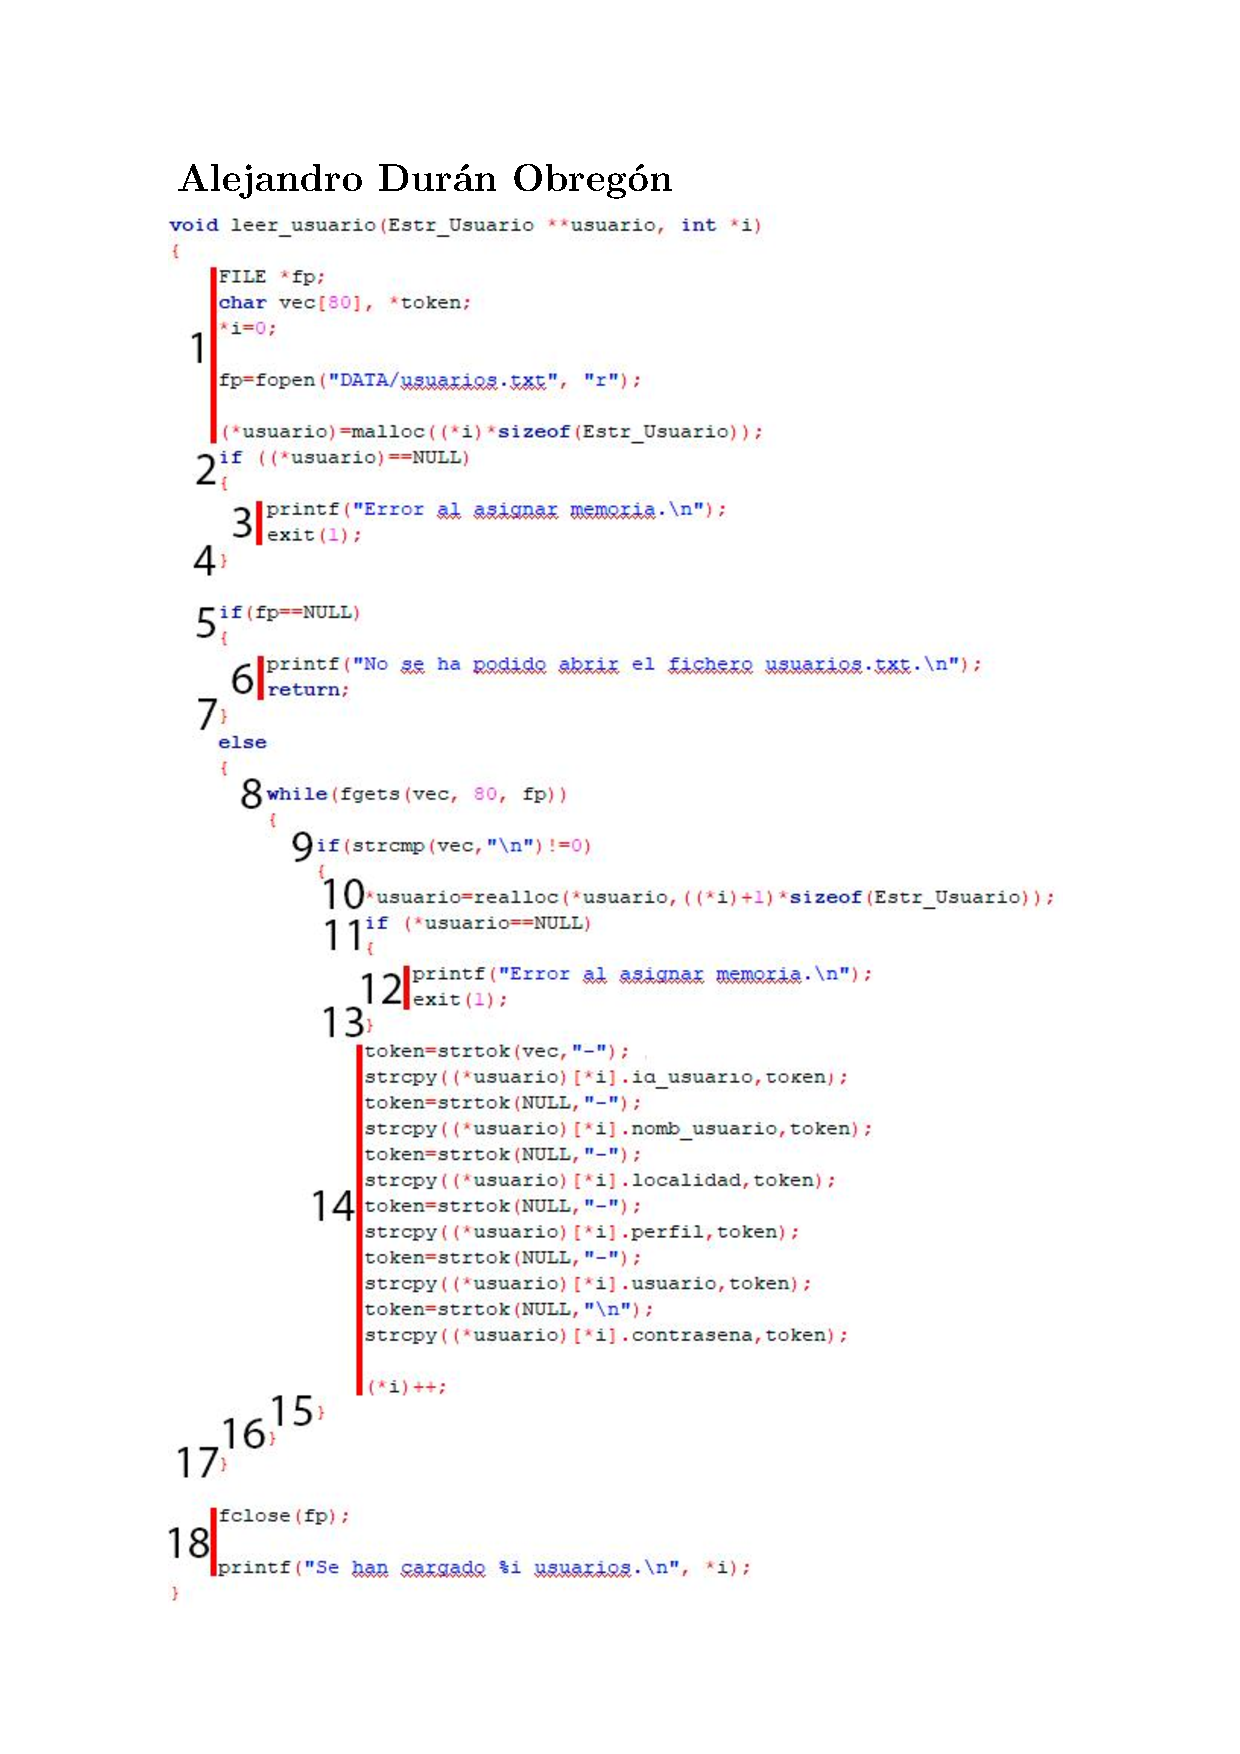
\includepdf[pages={1, 2, 3}]{FOTOS/Pruebas_Alejandro_Duran_Obregon.pdf}

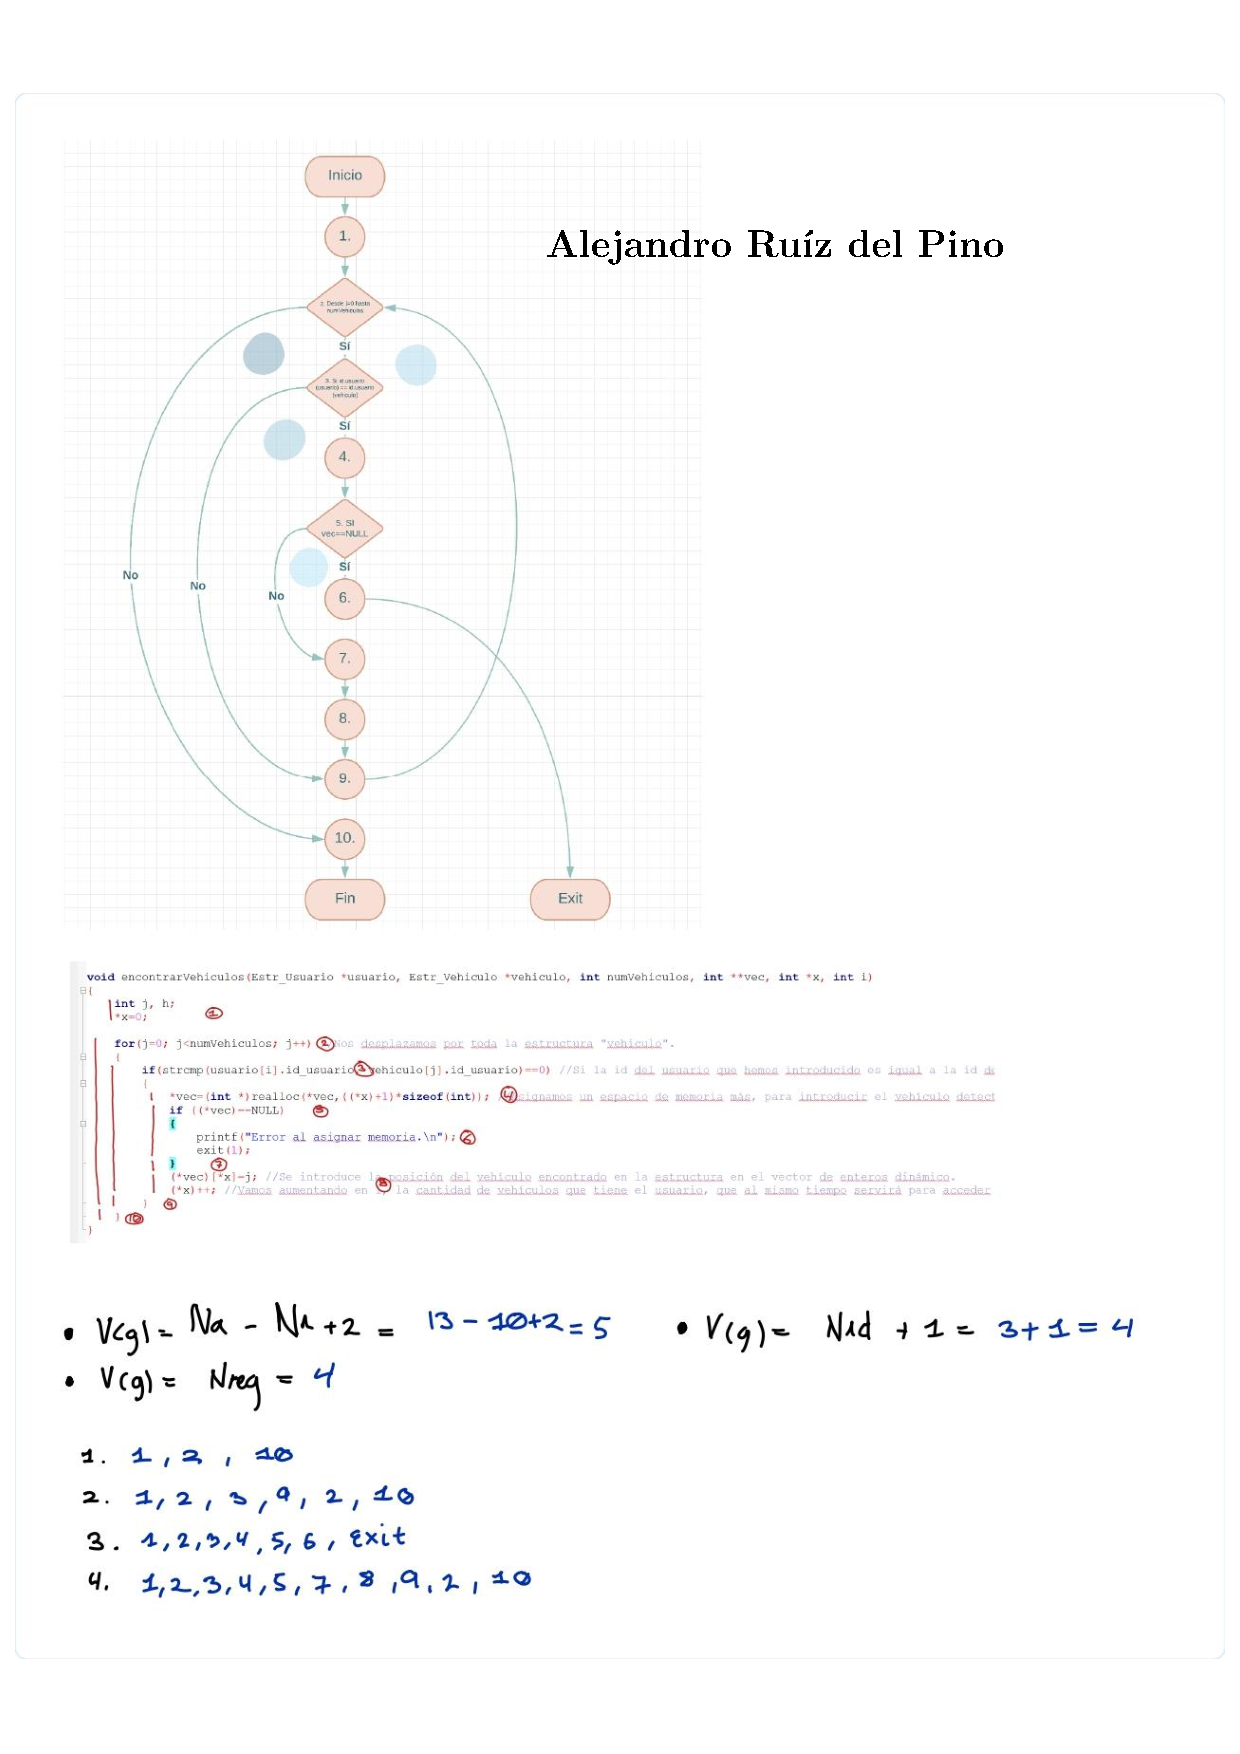
\includepdf[pages={1, 2}]{FOTOS/Pruebas_Alejandro_Ruiz_del_Pino.pdf}

\subsubsection{Plan de pruebas de aceptación}

En esta sección, se va a definir algunas rutas con las que usted podrá probar todos los puntos del programa. No se ha establecido una serie de datos específicos, para que así pueda probar con
todo lo que le guste, para poner a prueba el programa.

Primeramente, se encontrará el menú principal, en el que podrá acceder con las credenciales sugeridas en \ref{fig:menuPrincipal}, o puede registrar un nuevo usuario.
\begin{center}
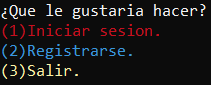
\includegraphics[]{FOTOS/menuPrincipal.png}
\end{center}
Empezaremos con el apartado de \textbf{Usuario}, introduciendo \textbf{usua1}, como usuario, y \textbf{2023}, como contraseña. 
Tras esto, se dirigirá al menú de \textbf{Pasajero}, introduciendo 1, podrá entrar en la parte de \textbf{Perfil}, en el que puede ver todos sus datos personales,
aquí puede modificar cualquier tipo de dato personal, verá que estos se actualizarán tanto en el fichero como en la estructura. Puede probar si estos se introducen correctamente, etc.
\begin{center}
    \begin{center}
      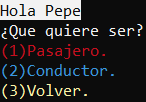
\includegraphics[]{FOTOS/menuSeleccionUsuario.png}
    \end{center}
    \begin{center}
      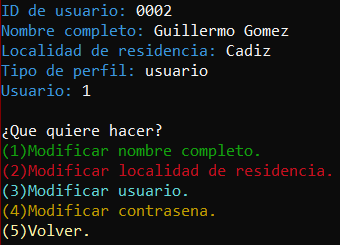
\includegraphics[]{FOTOS/menuPasajeroPerfil.png}
    \end{center}
\end{center}

Después, pulsará 2, para acceder al apartado de \textbf{Viajes}, donde podrá ver todos los viajes que tiene reservados, tras esto, puede probar las acciones del menú,
para poner a prueba el programa. Puede ver que el usuario sólo puede reservar viajes que pasan por su localidad de residencia, al igual que
no puede reservar dos veces en el mismo viaje, o que no le deja introducir una fecha anterior a la actual, etc.
\begin{center}
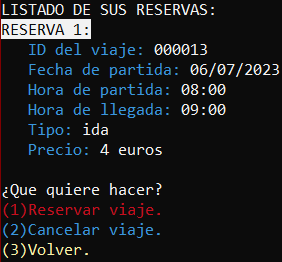
\includegraphics[]{FOTOS/menuPasajeroViaje.png}
\end{center}

Habiendo probado que todo funciona, puede volver al menú de selección de puesto, para escoger la opción de \textbf{Conductor}, introduciendo 1, entrará en el menú de \textbf{Perfil}, similar al anterior. 
\begin{center}
    \begin{center}
      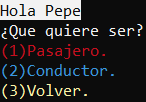
\includegraphics[]{FOTOS/menuSeleccionUsuario.png}
    \end{center}
    \begin{center}
      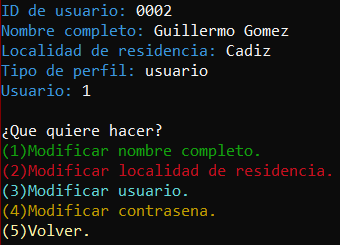
\includegraphics[]{FOTOS/menuPasajeroPerfil.png}
    \end{center}
\end{center}

Al haber probado esto, puede pulsar 2, para dirigirse al menú de \textbf{Vehículos}, donde tendrá a su vista un listado con todos los vehículos, que tiene registrados en el sistema, si lo desea,
puede explorar los menús y realizar diferentes acciones para probar el sistema, creando nuevos vehículos, o modificando y eliminando los existentes. Aquí puede ver que al eliminar un vehículo,
se eliminarán tanto sus viajes, reservas y pasos.
\begin{center}
  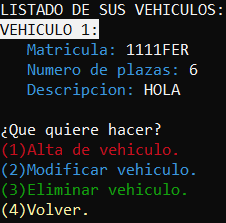
\includegraphics[]{FOTOS/menuConductorVehiculo.png}
\end{center}
Tras esto, puede dirigirse al menú de \textbf{Viajes}, introduciendo un 3, donde verá una lista de todos los viajes abiertos o iniciados que tiene en el momento, puede crear algún viaje,
para probar el sistema de creación de los mismos, o incluso modificar o anular o eliminar cualquiera. Sólo podrá anular viajes que estén abiertos, sin ninguna plaza ocupada, o finalizar,
viajes que ya estén iniciados.
\begin{center}
  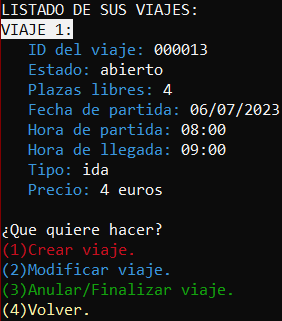
\includegraphics[]{FOTOS/menuConductorViaje.png}
\end{center}

\newpage

En segundo lugar, puede volver al menú principal, e introducir \textbf{admin}, como usuario, y \textbf{1234}, como contraseña. 
\begin{center}
    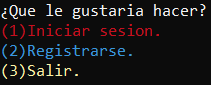
\includegraphics[]{FOTOS/menuPrincipal.png}
\end{center}

Tras esto, aparecerá un menú con 3 apartados, en \textbf{Usuarios}, podrá realizar diferentes funciones, como la creación de un usuario nuevo, o la eliminación de cualquier usuario existente,
al igual que puede modificarlos, y ver todos los usuarios del sistema, estas funciones trabajan de forma similar a las del usuario normal. 
\begin{center}
    \begin{center}
      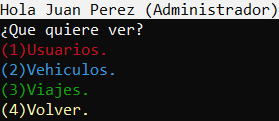
\includegraphics[]{FOTOS/menuAdmin.png}
    \end{center}
    \begin{center}
      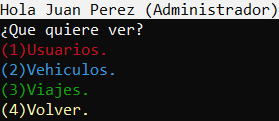
\includegraphics[]{FOTOS/menuAdmin.png}
    \end{center}
\end{center}

\newpage

Más tarde, podrá probar todo en el apartado de \textbf{Vehículos}, como la creación de nuevos vehículos al perfil de cualquier usuario, o la modificación o eliminación de vehículos existentes,
además, podrá ver una lista con todos los vehículos que hay en el sistema, o incluso ver un historial de los viajes que ha hecho un coche. 
\begin{center}
  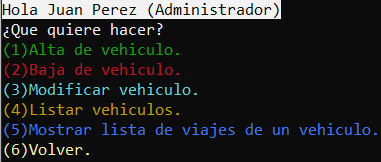
\includegraphics[]{FOTOS/menuAdminVehiculo.png}
\end{center}

Una vez haya terminado de probar todo, puede dirigirse al menú de \textbf{Viajes}, para crear un viaje con cualquier usuario del sistema, también podrá eliminar, anular o modificar
cualquier viaje que haya en la base de datos, al igual que podrá ver una lista de todos los viajes que han hecho cada usuario del sistema.
\begin{center}
  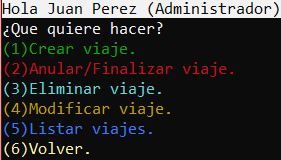
\includegraphics[]{FOTOS/menuAdminViaje.png}
\end{center}